\documentclass[12pt]{book}
\usepackage{amsmath,amsthm,amssymb,amsfonts,enumerate,mymath,tikz-cd,fancyhdr}
\openup 5pt
\author{Blake Farman\\University of South Carolina}
\title{Math 116\\Homework 04}
\date{October 18, 2016}
\pdfpagewidth 8.5in
\pdfpageheight 11in
\usepackage[margin=1in]{geometry}

\theoremstyle{definition}
\newtheorem{thm}{}
\renewcommand{\qedsymbol}{}

\begin{document}
\maketitle

\section*{5.2}

\setcounter{thm}{1}
\begin{thm}
Evaluate
\begin{enumerate}[(a)]
  \item 
    $\displaystyle{\cos(12\pi)}$
  \item
    $\displaystyle{\sin\left(\frac{5\pi}{2}\right)}$
  \item
    $\displaystyle{\sin\left(\frac{-9\pi}{2}\right)}$
  \item
    $\displaystyle{\cos(101\pi)}$
\end{enumerate}
\end{thm}

\setcounter{thm}{3}
\begin{thm}
  What is $\cos(\theta + \pi)$ in terms of $\cos(\theta)$? (Hint: Use the unit circle).
\end{thm}

\setcounter{thm}{5}
\begin{thm}
  \begin{enumerate}[(a)]
  \item
    In the triangle shown, calculate $\sin(\theta)$ and $\cos(\theta)$.
  \item
    Calculate $\sin^2(\theta) + \cos^2(\theta)$.

    \begin{center}
      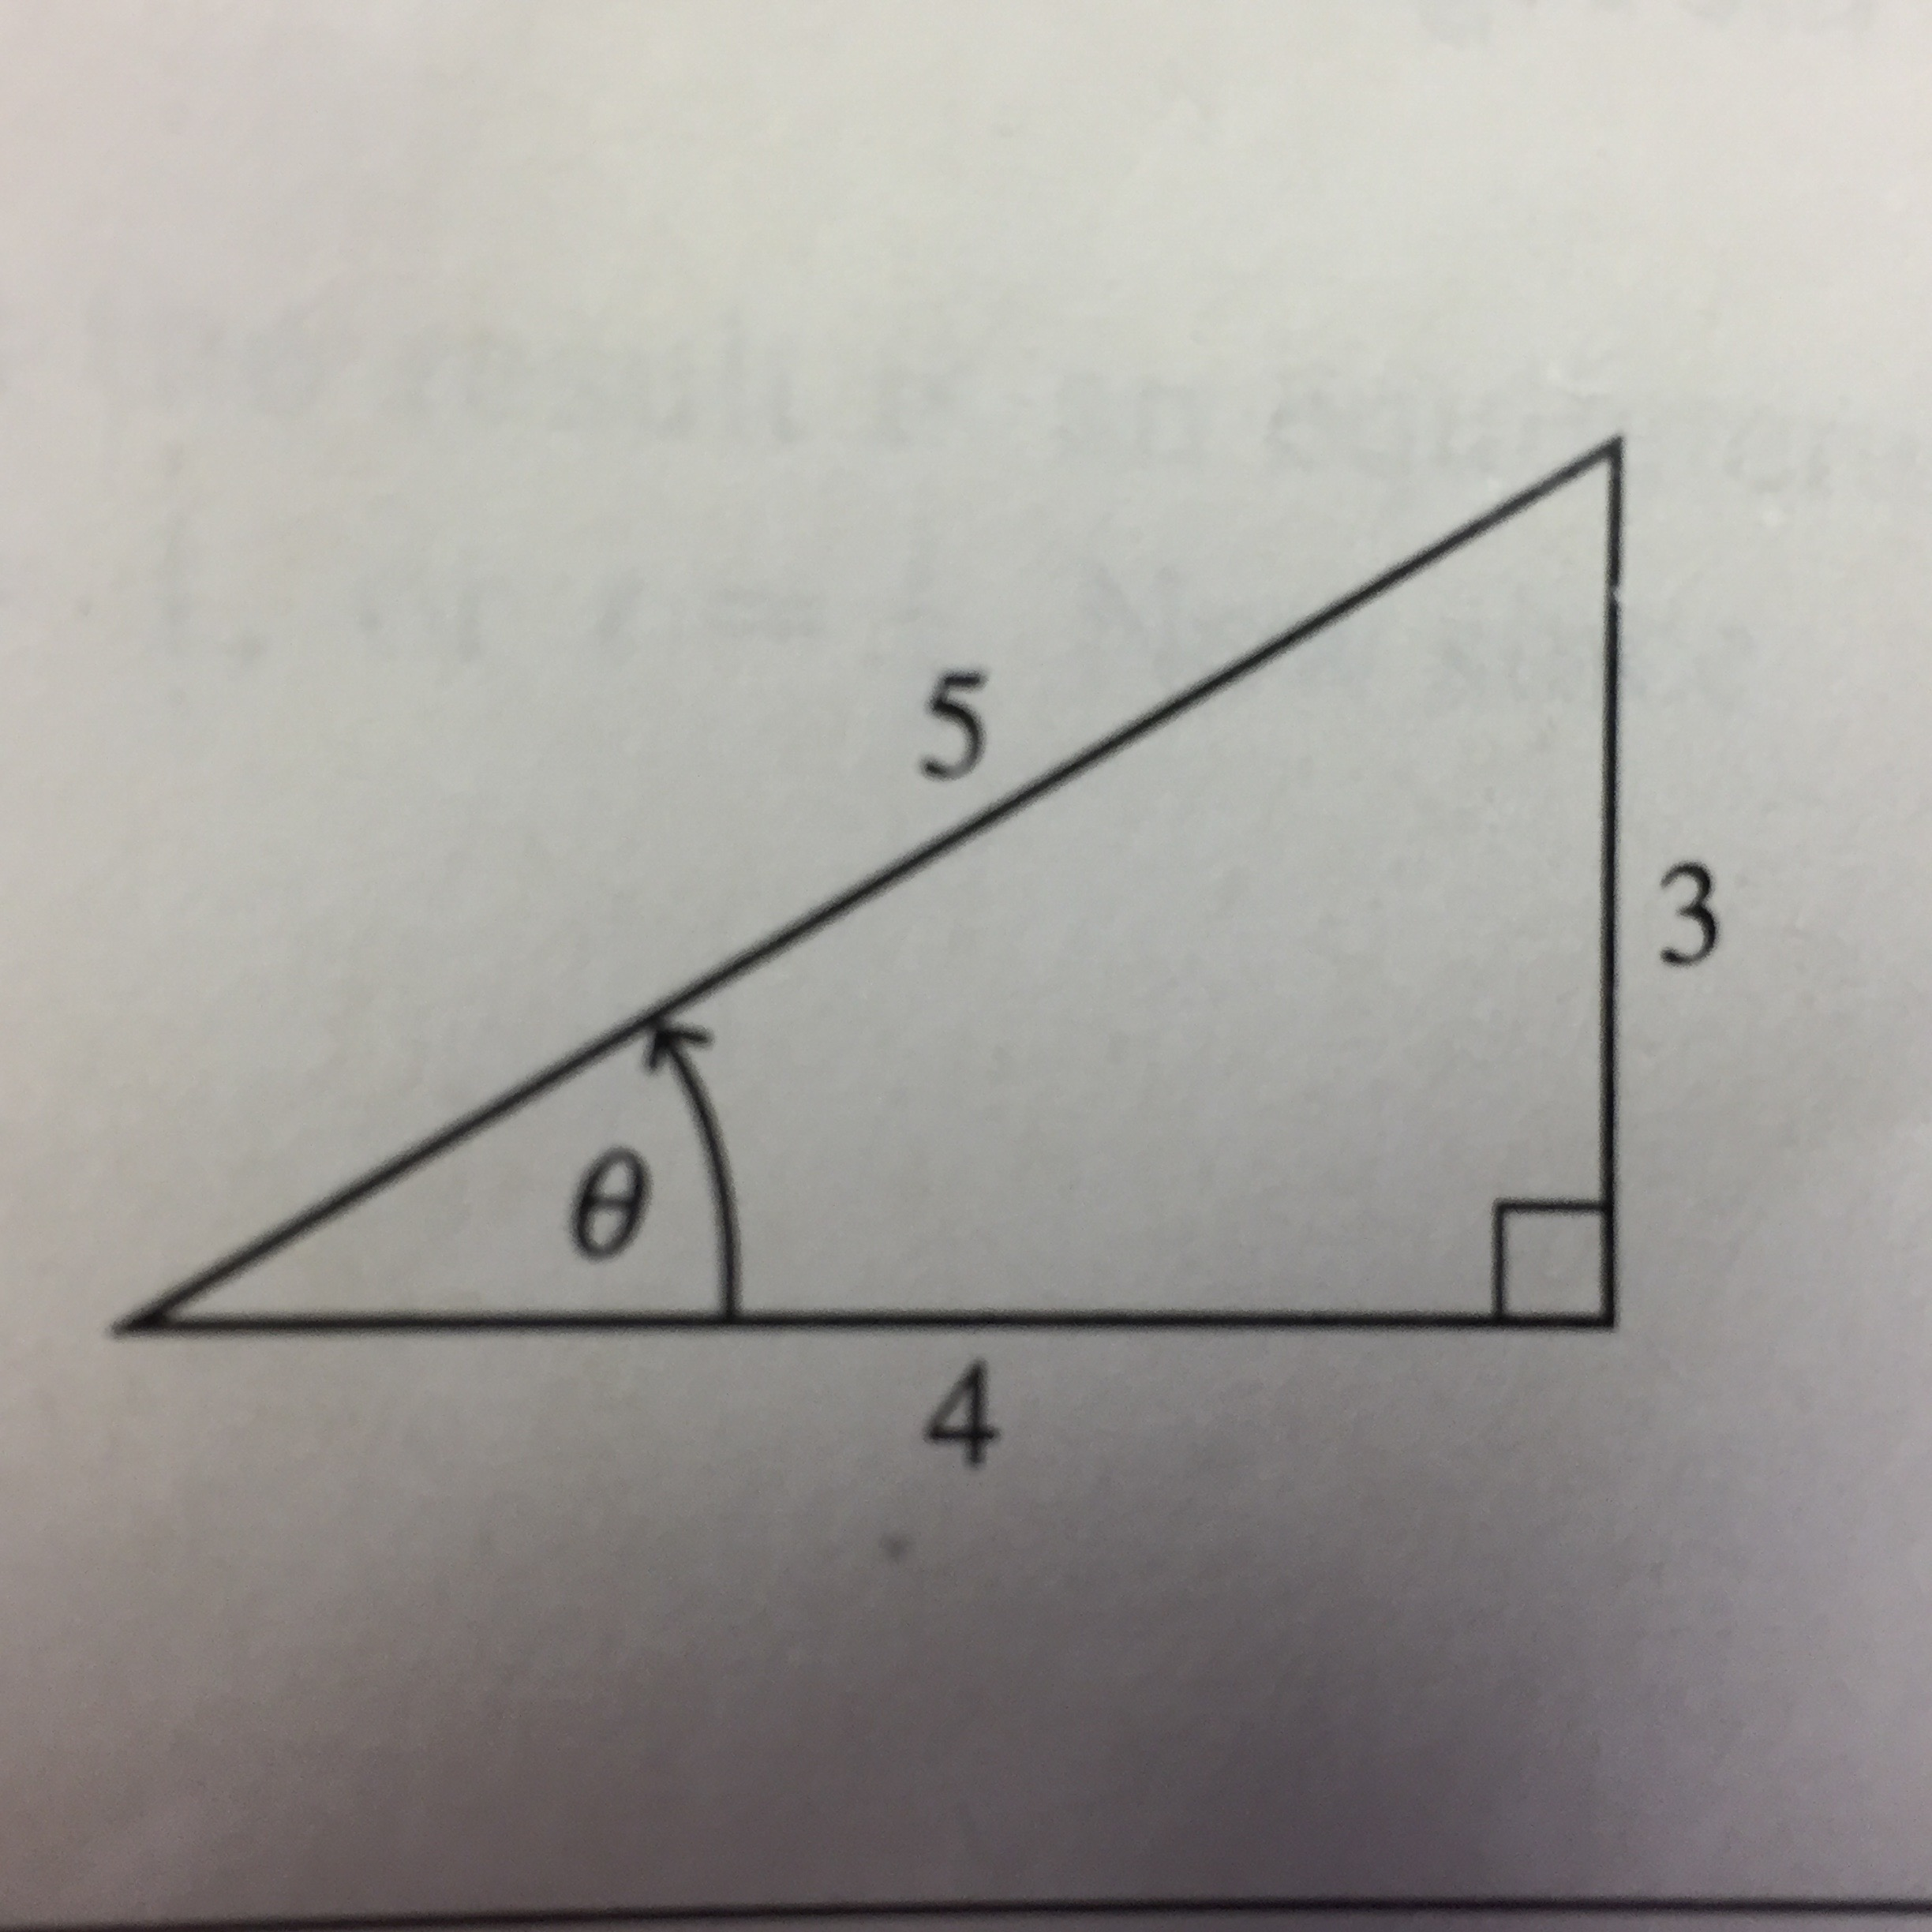
\includegraphics[scale=0.05]{triangle.jpg}
    \end{center}
  \end{enumerate}
\end{thm}

\section*{5.3}
Evaluate the following.

\setcounter{thm}{1}
\begin{thm}
  $\displaystyle{\sin\left(\frac{7\pi}{4}\right)}$.
\end{thm}

\setcounter{thm}{3}
\begin{thm}
  $\displaystyle{\cos\left(\frac{-3\pi}{4}\right)}$.
\end{thm}

\setcounter{thm}{7}
\begin{thm}
  $\displaystyle{\cos\left(\frac{13\pi}{6}\right)}$.
\end{thm}

\setcounter{thm}{11}
\begin{thm}
  $\displaystyle{\sin\left(\frac{29\pi}{6}\right)}$.
\end{thm}

\end{document}
